% =====================================================================
%  One Stack, Two Ledgers
%  CollusionGraph -- research paper, written from docs/paper_blueprint.md
%
%  COMPILING ON OVERLEAF
%  ---------------------
%  Upload this .tex together with the folder paper/figures/, which holds the
%  six vector figures (regenerate them with
%  `uv run python scripts/paper_figures.py`):
%      figures/fig1_architecture.pdf      figures/fig4_transfer_lift.pdf
%      figures/fig2_two_ledgers.pdf       figures/fig5_label_noise.pdf
%      figures/fig3_timestep_crater.pdf   figures/fig6_label_efficiency.pdf
%  Everything else is self-contained -- the tables are inlined, so there
%  is nothing to \input and no external .bib to resolve.
%
%  HOUSE RULE: every number in this paper is traced to an artifact under
%  eval_outputs/ via docs/reproducibility.md. Regenerate the tables with
%  `uv run poe paper-tables` before editing any figure quoted here.
% =====================================================================
\documentclass[conference]{IEEEtran}
\IEEEoverridecommandlockouts

\usepackage{cite}
\usepackage{amsmath,amssymb}
\usepackage{graphicx}
\usepackage{booktabs}
\usepackage{array}
\usepackage{xcolor}
\usepackage{balance}
\usepackage[hidelinks]{hyperref}
\usepackage{url}

\newcommand{\RQ}[1]{\textbf{RQ#1}}
% Revision marker: a number or claim that waits for a named run (revision-plan.md).
% It prints in red, and the final audit fails while any \PENDING remains.
\newcommand{\PENDING}[1]{\textcolor{red}{\textbf{[PENDING: #1]}}}

\begin{document}

\title{One Stack, Two Ledgers:\\
Budget-Evaluated, Explainable Collusion Screening\\
Across Illicit-Finance and Procurement Networks}

% All five authors share one affiliation, so IEEE style puts them in a single
% centred block with the institution stated once. The e-mail addresses are
% compressed on the shared @spjain.org domain, which is the conventional way to
% keep a five-author list on two lines.
\author{%
\IEEEauthorblockN{Rachit Garg, Kartik Joshi, Prem Kukreja, Gagandeep Singh,
and Samuel Alex}
\IEEEauthorblockA{\textit{SP Jain School of Global Management}\\
Dubai, United Arab Emirates\\
\texttt{\{rachit.garg,\,kartik.as25dxb025,\,prem.as25dxb029,\,gagandeep.as25dxb032,}\\
\texttt{samuel.as25dxb031\}@spjain.org}}
}

\maketitle

\begin{abstract}
Money laundering and bid rigging are studied by separate communities, yet both
are collusive crimes. No single transaction or tender looks wrong by itself;
the scheme shows only in the pattern of dealings around it. We built one
graph-learning stack for both domains. A single intermediate representation
feeds one detector family, one explanation layer and one evaluation protocol,
and six adapters carry five public datasets into it. Under strict inductive
splits and fixed alert budgets, gradient-boosted trees on graph features beat
every graph neural network we trained on Elliptic++. Over five seeds each, the
trees score $0.8123 \pm 0.0012$ AUC-PR against $0.4729 \pm 0.0525$ for
GATv2-focal, and the gap holds on every seed pair. The whole gap lies before a
market closure at time step 43; after it, both models fall close to the base
rate. Transfer between procurement markets is uneven. All four Garc\'ia markets
beat their base rate, with a pooled lift of $1.36$, but the pooled lift over
the seven Mendeley countries is $0.93$. Across domains, a frozen procurement
encoder reaches $0.150$ AUC-PR on Elliptic++ against a base rate of $0.065$,
while a linear probe on the target's own features reaches $0.299$. The reverse
direction falls below its base rate.
\PENDING{B7: the label-noise and regulariser result}
The released system ranks group alerts for a fixed review budget, explains
each alert with a subgraph and a red-flag citation, and leaves every decision
to a human reviewer.
\PENDING{L3: repository-availability wording, an author decision}
\end{abstract}

\begin{IEEEkeywords}
graph neural networks (GNN), anomaly detection, anti-money laundering (AML), bid rigging, class imbalance, transfer learning, evaluation protocol.
\end{IEEEkeywords}

% =====================================================================
\section{Introduction}
% =====================================================================

Money laundering and bid rigging are screened by two enforcement worlds that
have never shared a toolchain. Inside banks, anti-money-laundering (AML) teams
run transaction-monitoring rules that fire on individual records. Most of the
resulting alerts are false positives: a CEPS task force puts their share
often at around 95--98\%~\cite[pp.~3, 31]{lannoo2021}. Competition authorities and
procurement officials face the opposite problem. Bid-rigging agreements are
typically negotiated in secret and are hard to detect~\cite[p.~23]{oecd2025}.
Detection therefore leans on red flags spotted in tenders and on self-reporting
through leniency and whistleblower programmes~\cite[pp.~12, 14]{oecd2025}.

The two problems are closer than they appear. A single small wire transfer
looks unremarkable, but twelve accounts passing the same money around a circle
within 72 hours is a laundering pattern. A single bid can be clean: the tender
was advertised, the bids arrived and a winner was declared. Yet five firms that
quietly take turns winning, whose losing bids sit suspiciously close in price
and who share directors and an address, may form a cartel. In both cases each
record looks innocent on its own, and the participants keep every record below
the thresholds the rules check. The scheme shows only in the network of
dealings. Confirmed cases are also rare against the volume of normal activity.

Fig.~\ref{fig:ledgers} makes the correspondence concrete. Five mechanisms recur
across the two domains, and each collapses to one graph signature. Laundering
cycles and bid rotation are directed cycles. Smurfing and cover bidding are
fan-in stars. Layering and market allocation are fan-out stars. Shell-company
chains and shared directorships form dense subgraphs of common attributes.
Pass-through clusters and closely grouped bid prices form tight communities
with unusual edge attributes. If the correspondence holds, one model can serve
both ledgers. We can then measure whether a learned notion of collusion
structure carries over between them, instead of assuming that it does.


\begin{figure*}[t]
\centering
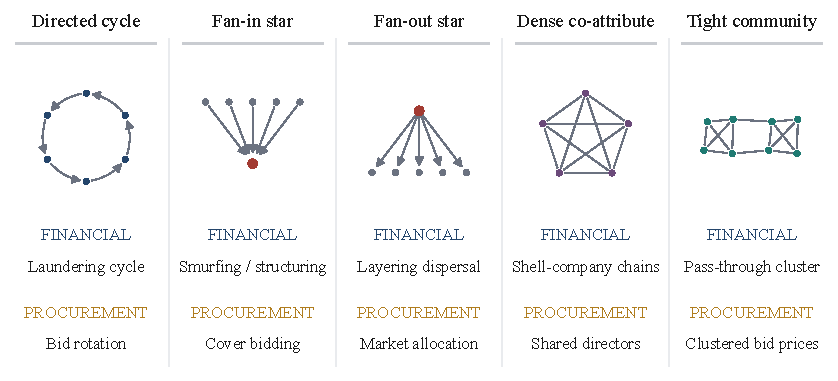
\includegraphics[width=\textwidth]{figures/fig2_two_ledgers.pdf}
\caption{Two ledgers, one structure. Five collusion mechanisms, the graph
signature each leaves behind, and the domain-specific name it goes by on
either side. The correspondence is the premise of the shared stack: only the
adapters and the red-flag vocabularies differ below it.}
\label{fig:ledgers}
\end{figure*}

A screening tool in either world is also held to a rising standard of
accountability. For high-risk AI systems, the EU AI Act requires automatic
logging, enough transparency for deployers to interpret the output, and
effective human oversight~\cite[Arts.~12--14]{aiact}. For stand-alone
Annex~III systems these requirements apply from 2~December
2027~\cite{omnibus}. We treat them as the standard a screening tool should
meet, not as a legal obligation that this system has been shown to face. An
AML screener does not assess creditworthiness, so it generally falls outside
Annex~III point~5(b)~\cite{aiact,eccguidance}. Section~\ref{sec:regulatory}
maps each requirement onto a property of the system.

\subsection{Research questions}

\begin{itemize}
\item[\RQ{1}] Can graph neural networks combined with unsupervised graph
anomaly detection identify illicit-finance and bid-rigging structures with
materially higher precision \emph{at fixed alert budgets} than rule-based and
tabular machine-learning baselines?
\item[\RQ{2}] Do models trained on confirmed cases beat the base rate in
unseen procurement markets, and which planted collusion motifs can
unsupervised detectors recover at a fixed budget?
\item[\RQ{3}] How faithful are the subgraph explanations of the alerts, and
how many alerts match a red-flag pattern that practitioners already use?
\item[\RQ{4}] Does a representation of collusion structure learned in one
domain provide usable signal in the other?
\end{itemize}

\subsection{Contributions}

The paper makes two contributions.

\begin{enumerate}
\item \textbf{A budget-first, leakage-safe evaluation protocol.} It combines
strict inductive splits, frozen train-time normalisation, tie-aware
precision@$k$, multi-seed reporting and paired stratified bootstrap tests. A
leakage test suite enforces it in continuous integration, and a
number-to-config map traces every reported figure. We count the protocol as a
contribution because the recent critiques of graph-anomaly evaluation are
implemented here, not only cited.
\item \textbf{A unified cross-crime representation with transfer
measurements.} One intermediate representation and six adapters carry five
public datasets from both domains. The awkward parts of each dataset are
recorded rather than patched over: missing bidder identities, case-control
sampling and a post-window label spike. On this representation we measure
transfer between procurement markets and between the two domains.
\end{enumerate}

Two further results support these contributions. The first is a catalogue of
negative results, including \PENDING{B7: count of supporting measurements}
measurements showing that validation selection cannot see the Elliptic
distribution shift. The second is an explanation layer and a guarded copilot,
released with the code.

% =====================================================================
\section{Related Work}
% =====================================================================

\textbf{Graph anomaly detection and benchmarks.} The survey by Ma et
al.~\cite{ma2023} supplies the node/edge/subgraph taxonomy we work inside.
GADBench~\cite{gadbench} is the uncomfortable reference point. Across 29
models and ten datasets, tree ensembles with plain neighbourhood aggregation
match or beat graph neural networks designed for the task. BOND~\cite{liu2022bond}
benchmarks the unsupervised detectors in the same way. Our \RQ{1} result shows
the same pattern on Elliptic++ under a strict protocol, which makes the
reproduction worth reporting.

\textbf{AML with graph neural networks.} Motie and Raahemi~\cite{motie2024}
survey the field. LineMVGNN~\cite{linemv2025} adds a line-graph view to two-way
message passing so that direction of money flow is preserved. On the original
Elliptic data, Weber et al.\ found that a random forest beat their graph
convolutional network. They also found that every method, the random forest
included, failed after a dark-market shutdown at time step 43~\cite{weber2019}.
Our \RQ{1} result confirms both findings under a stricter protocol.
LaundroGraph learns self-supervised representations of customer--transaction
graphs for anti-money laundering~\cite{cardoso2022}. Egressy et al.\ add
reverse message passing, port numbering and ego identifiers to standard
message passing. On anti-money-laundering data they report gains of up to
30\% in minority-class F1~\cite{egressy2024}. Removing the reverse edges from
our direction-aware graphs costs $0.194$ AUC-PR, the largest single-component
effect we measured. Near-perfect Elliptic results are best read with the ablations in the same
papers. One wavelet-temporal graph transformer reports about $0.98$
accuracy~\cite{lin2026}. The same paper notes that its wavelet features
contribute roughly $0.01$ and are ``not strictly indispensable''.

\textbf{Cartel detection.} The screens tradition of coefficient of variation,
price spread and kurtosis is long established and has been tested on real
cartel cases~\cite{imhof2018}. Huber and Imhof combine such screens with
machine learning~\cite{huber2019}, and statistical tests can single out groups
of colluding bidders~\cite{conley2016}. Corruption-risk indicators built from
procurement records~\cite{fazekas2020} and network analyses of contracting
markets~\cite{wachs2021} extend the approach to corruption more broadly. The
benchmarks that get reused come from Garc\'ia Rodr\'iguez et
al.~\cite{garcia2022} and the Mendeley EU cartel release~\cite{mendeley2025}. Recent cartel GNN work posts strong
cross-market numbers. Graph attention networks over tender--firm graphs from 13
markets in seven countries transfer at 80--90\% accuracy~\cite{imhof2025}. They
peak at 91\% on an eight-market configuration and settle at 84\% once extended
to 12 markets. Relational GCNs with an explicit zero-shot phase attack
out-of-distribution generalisation head on~\cite{gomes2024}, and a systematic
mapping study finds few methods applied in real systems to detect new
cases~\cite{epjds2025}. Those
accuracy figures and our budget-first lift numbers are different metrics on
differently sampled data, so we make no claim to beat them. What our matrices contribute is the shape of the degradation. It is
uneven across markets, and on the harder of the two benchmarks the market that
fails is the biggest one.

\textbf{Evaluation-protocol critiques.} A recurring complaint is that
machine-learning results, graph results among them, are inflated by
leakage~\cite{kaufman2012,kapoor2023} and by evaluation on a single fixed
split~\cite{shchur2018}. A third problem is a mismatch between the unit that
gets scored and the unit a human reviews. Our
transaction-versus-actor disagreement in Section~\ref{sec:granularity} measures
the third of those directly.

\textbf{Transfer and graph foundation models.} The graph-foundation-model
literature asks whether one representation can serve many
graphs~\cite{liu2025gfm,mao2024}. Pre-training on graph structure can transfer
across graphs~\cite{qiu2020gcc}, but it can also transfer
negatively~\cite{hu2020}. \RQ{4} puts
that question to two enforcement domains in a form that can come back negative,
and in one direction it does.

\textbf{LLM-augmented explanation.} Several groups now pair language models with
graph explanations to produce narratives an analyst can read~\cite{cedro2026}.
Retrieval ties generated answers to source records~\cite{lewis2020}, but
hallucination remains a known risk~\cite{ji2023}. We kept ours on a
short leash: read-only SQL over published artifacts, a numeric sanity gate, and
a guard on guilt-attributing language. The aim is an assistant that helps a
reviewer participate without inviting them to defer.

% =====================================================================
\section{Data and Unified Representation}
% =====================================================================

\subsection{Datasets}

Table~\ref{tab:data} lists the five public datasets in the six graph views our
six adapters build from them. Elliptic++ supplies both a transaction graph and
an actor graph, and the disagreement between the two is itself a result
(Section~\ref{sec:granularity}). Two views are labelled anchors carrying the
headline results. The rest supply scale, controllable ground truth, and an
unlabelled population for injection studies. Every dataset is
downloaded from its canonical source and verified against a committed
checksum manifest that also records its licence. No raw data is redistributed
in the release.

\begin{table*}[t]
\caption{Five public datasets in the six graph views the adapters build.
Roles: \textsc{anchor} carries headline results, \textsc{scale} stresses the
pipeline, \textsc{population} supplies an unlabelled portfolio for injection.
Positives are quoted in each dataset's own unit --- see
Section~\ref{sec:prevalence} for which denominator each evaluation uses.}
\label{tab:data}
\centering
\footnotesize
\setlength{\tabcolsep}{2.5pt}
\begin{tabular}{llllll}
\toprule
Dataset & Domain & Scale & Positives & Role & Licence \\
\midrule
Elliptic++ (tx graph)~\cite{elmougy2023,weber2019} & Financial & 203,769 nodes, 234,355 edges, 49 steps & $\approx$2\% illicit & \textsc{anchor} & research use \\
Elliptic++ (actor graph)~\cite{elmougy2023} & Financial & test window: 292,102 wallets, 966,352 edges & 5.3\% (test window) & granularity & research use \\
IBM AMLworld HI-Small~\cite{altman2023} & Financial & 5,078,345 tx, 515,088 accounts & 0.102\% laundering & \textsc{scale} & CDLA-Sharing-1.0 \\
Mendeley EU cartel~\cite{mendeleydata2025} & Procurement & 15,616 contracts, 7 countries, 2004--21 & 41.9\% (case-control) & \textsc{anchor} & CC BY-NC 3.0 \\
Garc\'ia Rodr\'iguez et al.~\cite{garcia2022} & Procurement & 64,348 bids, 9,781 tenders, 6 markets & 11.3--81.8\% by market & transfer & CC BY-NC-ND 4.0 \\
OCDS Georgia (OpenTender) & Procurement & 163,327-node window & unlabelled & \textsc{population} & CC BY-NC-SA 4.0 \\
\bottomrule
\end{tabular}
\end{table*}

\subsection{The intermediate representation}

Every adapter emits the same typed structure: nodes, directed attributed edges,
labels carrying provenance and confidence, and a history pack that supports
as-of feature computation. Everything downstream is then domain-agnostic. The
contract also forbids cleaning heroics. An adapter may not impute a missing
identity, invent an edge, or quietly drop an inconvenient property of the
source. Three such properties survive into the representation as a result.

\begin{itemize}
\item \textbf{Garc\'ia bidder identities exist on four of six markets.} The
company-identifier column appears only in the per-market files for Japan, Italy,
Brazil and the USA. The combined file drops it, and the two Swiss markets never
carried it at all. Co-bidding \emph{identity} graphs are buildable on four
markets; the rest support only the anonymous bid-price tier.
\item \textbf{Mendeley is a case-control research sample}, not a population
file, and 41.9\% of its contracts are cartel-linked. Raw AUC-PR therefore
cannot be compared across its folds, whose prevalences run from $0.29$ to
$0.89$. Throughout this paper the cross-fold comparator is lift over fold
prevalence, never raw AUC-PR.
\item \textbf{AMLworld has a post-window label spike.} Of the transactions
dated after 10 September, 1,108 in number, 59.1\% are laundering, some 580
times the base rate. Our temporal splitter fences that tail off explicitly. A
naive split would produce a spectacular number and a meaningless one.
\end{itemize}

\subsection{A note on which prevalence is being quoted}
\label{sec:prevalence}

Three different denominators circulate in the literature on these datasets.
Mixing them up can make a result look better or worse than it is. We
therefore fix the convention here and keep it for the rest of the paper.

Take Elliptic++ first. About 2\% of all transactions are labelled illicit, but
77\% carry no label whatsoever. We compute every metric over confirmed nodes
only, and in the test window of steps 35--49 that confirmed-only prevalence is
$0.065$. This is the baseline our AUC-PR should be read against and the figure
quoted in Table~\ref{tab:t1}. The 2\% describes the dataset; $0.065$ describes
the evaluation.

AMLworld splits by unit instead of by labelling. Laundering accounts for
0.102\% of transactions, while account-level node prevalence in our test split
is $0.0103$. Since our baselines score accounts, $0.0103$ is the number that
matters in Section~\ref{sec:robustness}.

Mendeley splits the same way. Cartel-linked contracts make up 41.9\% of the
case-control sample; firm-level test prevalence is $0.358$. Every Mendeley
result we report is firm-level.

\subsection{As-of label and feature policies}

Any feature computed from a node's history is computed as of the split
boundary, never across the full record. We treat this as a contribution and not
an implementation footnote, because history-derived features are where temporal
leakage prefers to hide. Aggregate statistics will not reveal it. The only
symptom is a validation score that looks a little too good. A dedicated leakage
suite enforces the policies and runs as its own continuous-integration step on
every push.

% =====================================================================
\section{Method}
% =====================================================================

Fig.~\ref{fig:arch} shows the whole system. One design rule governs it: a hard
trust boundary. The offline pipeline writes plain files and exits. Everything
on the user-facing side is read-only and can neither retrain a model nor alter
a score.

\begin{figure*}[t]
\centering
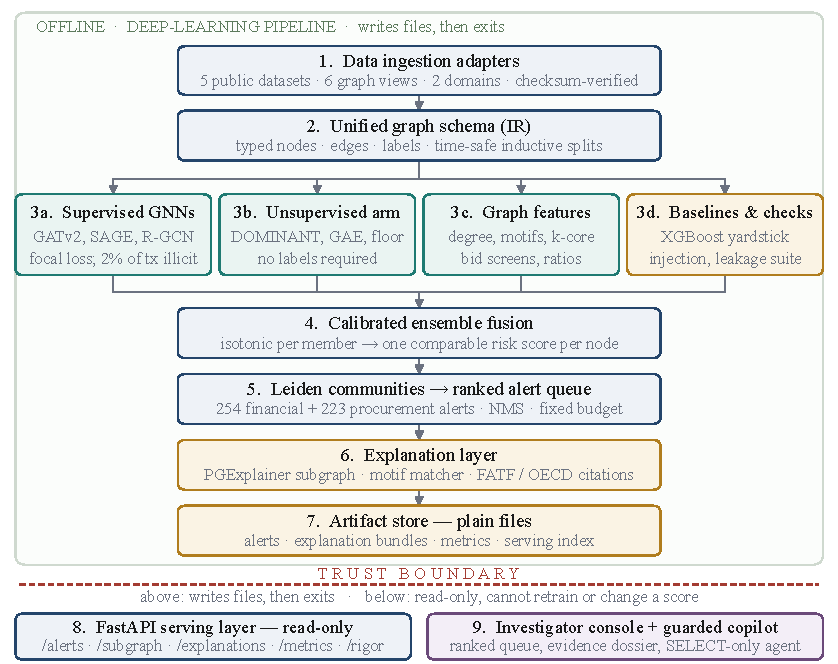
\includegraphics[width=\textwidth]{figures/fig1_architecture.pdf}
\caption{The shared stack. Stages 1--7 run offline and terminate, writing
Parquet and JSON artifacts; stages 8--9 serve those artifacts read-only. The
same nine stages run for both domains; only the ingestion adapters and the
red-flag vocabularies differ.}
\label{fig:arch}
\end{figure*}

\subsection{Detection arms}

Four arms score every node and are fused afterwards.

\textbf{Baselines.} B1 is a rule engine in the spirit of the threshold logic
banks actually deploy. B2 is XGBoost~\cite{chen2016} on node features. B3 is XGBoost on node
features together with graph-derived ones, meaning degrees, k-core, motif counts
and neighbourhood aggregates. B3 follows the GADBench recipe and is the yardstick
that matters. On the procurement side we add B4, a transparent screens
composite over award screens: a firm's number of awards, its market share and
the concentration of its buyers. The bid-price screens of the cartel
literature need the losing bids, which the Mendeley release does not contain.

\textbf{Supervised graph neural networks.} GraphSAGE~\cite{sage},
GATv2~\cite{gatv2} and R-GCN~\cite{rgcn}, all direction-aware: the graph is
built with explicit reverse edges so that message passing can distinguish
sending from receiving. Focal loss~\cite{focal} is the default given the
imbalance; weighted cross-entropy is the ablation arm.

\textbf{Unsupervised arm.} DOMINANT~\cite{dominant} and a graph
autoencoder~\cite{kipf2016}
score structural reconstruction error, plus a deterministic structural floor.
These require no labels and are the only arms available on the unlabelled OCDS
population~\cite{ocds}.

\textbf{Fusion.} We isotonically calibrate~\cite{zadrozny2002} each member on
validation before
fusing, so the combined score behaves like a comparable probability instead of
an arbitrary blend of ranks. The gap between calibrated and rank fusion turned
out to be one of the largest effects we measured anywhere in the paper.

\subsection{From node scores to an alert queue}

What limits a compliance team is investigator hours, not model output, so the
operational unit has to be a group and not a node. Leiden community
detection~\cite{leiden} over the scored graph proposes the candidates. We then
rank groups by aggregate member risk, deduplicate them with Jaccard non-maximum
suppression, cap their size, and cut the list at a fixed review budget. A group
counts as a hit when at least one member is confirmed, tie-aware.
Section~\ref{sec:robustness} sweeps every parameter in that pipeline.

\subsection{Explanation layer}

For each alert the system returns four things. The first is the minimal
responsible subgraph from PGExplainer~\cite{pgexplainer}, which we adopted over
GNNExplainer~\cite{gnnexplainer} after the ablation in Section~\ref{sec:rq3}.
The others are the matched motif, the attributes supporting it, and the FATF or
OECD red-flag indicator that the shape corresponds to. An alert without an explanation does not count as delivered.

\subsection{Guarded copilot}

A bounded language-model agent answers analyst questions using the published artifacts. It is constrained by design. It has a SELECT-only allowlist over read-only views, a numeric check that rejects any figure absent from the rows it read, a guilt-language guard, and a disclaimer on every response. Its release gate is a golden set of 26 cases, graded for grounding and for violations in the released output. Anything that ships has zero tolerance; drafted rewrites have a separate limit.

\subsection{Evaluation protocol}
\label{sec:protocol}

Each rule below changed a headline number at some point while we built the system. We therefore treat the protocol as a result in its own right. Appendix~\ref{app:methods} gives every split, feature, rule and hyperparameter.

\begin{itemize}
\item \textbf{Strict inductive splits.} Test nodes and their edges stay unseen during training. Temporal splits fence the boundary; entity splits (LOCO, LOMO) hold out whole countries or markets.
\item \textbf{Frozen train-time normalisation.} We compute feature statistics on training and freeze them. Recomputing them on the test set is unintentional test-time adaptation. Removing it pulled our own headline GATv2 number down from
$0.693$ to $0.532$, which widened the gap to the tree baseline. Every figure we report is after the fix.
\PENDING{D24: replace with the five-seed per-graph normalisation measurement}
\item \textbf{Budget-first, tie-aware metrics.} We report tie-aware precision@$k$ at budgets a real team would use. We also report AUC-PR, the right summary under this level of class imbalance~\cite{saito2015}, always against its own fold’s prevalence baseline.
\item \textbf{Multi-seed with dispersion.} Five seeds, reported as mean~$\pm$~standard deviation. The seed variance, about $\pm 0.05$, is much larger than the cross-machine variance of about $\pm 0.02$, so a single-seed comparison between two machines is unreliable. Our own previously published seed-0 GATv2 figure of $0.5492$ happens to be the best of the five. The more reliable number is $0.4729 \pm 0.0525$, and that is the one we quote.
\item \textbf{Paired stratified bootstrap}~\cite{efron1993} over identical
confirmed test nodes
for every headline comparison, at 2,000 resamples.
\end{itemize}

% =====================================================================
\section{Results}
% =====================================================================

\subsection{RQ1: graph models do not beat the trees}

The answer to \RQ{1} is no. On neither anchor dataset, and at none of the
budgets we report, does a graph neural network or its fusion with unsupervised
detectors beat the tree baselines.

Table~\ref{tab:t1} gives the Elliptic++ scoreboard. Gradient-boosted trees on
graph features reach $0.8123 \pm 0.0012$ AUC-PR over five seeds, against a
prevalence of $0.065$. The best graph neural network we trained reaches
$0.4729 \pm 0.0525$. We paired each GATv2 seed with the tree seed of the same
index. The paired bootstrap puts the five differences between $-0.264$ and
$-0.391$, with every 95\% interval below zero and every $p$ at the resolution
floor (Table~\ref{tab:t3}). On scores averaged over the five seeds, the
difference is $-0.301$ (95\% CI $[-0.324, -0.276]$).

\begin{table}[t]
\caption{Elliptic++ node-level results (test steps 35--49, prevalence
$0.065$). The rule baseline is deterministic; tree, GNN and ensemble rows are
5-seed mean $\pm$ standard deviation. The two ``local'' rows use only the 94
local columns (the time step and 93 local features).}
\label{tab:t1}
\centering
\footnotesize
\setlength{\tabcolsep}{4pt}
\begin{tabular}{lll}
\toprule
Model & AUC-PR & P@100 \\
\midrule
B1 rules & 0.0576 (det.) & 0.00 \\
B2 XGBoost, local & $0.7879 \pm 0.0011$ & $1.00 \pm 0.00$ \\
B3 XGBoost + graph, local & $0.7959 \pm 0.0014$ & $1.00 \pm 0.00$ \\
B2 XGBoost & $0.8039 \pm 0.0017$ & $1.00 \pm 0.00$ \\
\textbf{B3 XGBoost + graph} & $\mathbf{0.8123 \pm 0.0012}$ & $\mathbf{1.00 \pm 0.00}$ \\
GATv2-focal & $0.4729 \pm 0.0525$ & $0.8120 \pm 0.2383$ \\
GATv2-weighted CE & $0.4388 \pm 0.0505$ & $0.7240 \pm 0.1466$ \\
DOMINANT & $0.0410 \pm 0.0003$ & --- \\
Ensemble, calibrated & $0.4434 \pm 0.0501$ & --- \\
Ensemble, rank & $0.0511 \pm 0.0019$ & --- \\
Structural floor & $0.0547 \pm 0.0000$ & --- \\
GAE & $0.0386 \pm 0.0001$ & --- \\
\bottomrule
\end{tabular}
\end{table}

\begin{table}[t]
\caption{Paired-bootstrap comparisons over identical confirmed test nodes
($n = 16{,}670$; 2,000 stratified resamples). ``Seed pairs'' rows give the
range of the five per-seed differences and the envelope of their intervals.
``Seed-averaged'' rows compare each model's score averaged over seeds 0--4.
Every $p$ value sits at the resolution floor of 2,000 resamples under add-one
smoothing ($2/2001 \approx 0.001$), so they should be read as $p < 0.001$
rather than as point estimates.}
\label{tab:t3}
\centering
\footnotesize
\setlength{\tabcolsep}{3pt}
\begin{tabular}{lrrr}
\toprule
Comparison & $\Delta$ AUC-PR & 95\% CI & $p$ \\
\midrule
\multicolumn{4}{l}{\textit{GATv2-focal vs.\ B3}} \\
\quad Seed pairs & $-0.264$ to $-0.391$ & $[-0.416, -0.238]$ & $<0.001$ \\
\quad Seed-averaged & $-0.301$ & $[-0.324, -0.276]$ & $<0.001$ \\
\multicolumn{4}{l}{\textit{Calibrated vs.\ rank fusion}} \\
\quad Seed pairs & $+0.342$ to $+0.471$ & $[0.314, 0.500]$ & $<0.001$ \\
\quad Seed-averaged & $+0.444$ & $[0.413, 0.474]$ & $<0.001$ \\
\bottomrule
\end{tabular}
\end{table}

Most of the trees' strength sits in the local transaction features. On the 94
local columns alone, B2 reaches $0.7879 \pm 0.0011$. The 72 neighbourhood
aggregates and the 17 Elliptic++ additions, which include in- and out-degree,
add $0.016$. Explicit graph features add about $0.008$ in both settings: B3
beats B2 on every seed, and B3-local beats B2-local by the same margin. The
graph therefore carries some signal for the trees. The deep models fail to turn
it into ranking quality, and their deficit appears before the market closure
discussed below.

Calibration matters only once members are fused. Rank fusion of the ensemble
members collapses to $0.0511 \pm 0.0019$, while calibrated fusion reaches
$0.4434 \pm 0.0501$ (Table~\ref{tab:t1}). Calibrated fusion is therefore
necessary if members are fused, but it did not beat its best member:
GATv2-focal alone scores $0.4729 \pm 0.0525$. GATv2 is the only supervised
member of the fusion, and removing the unsupervised members raises the
ensemble by $0.0295$ (Table~\ref{tab:t7}). Adding B3 to a calibrated fusion does
not help either. B3 must then train on steps 1--29, so that steps 30--34 can
fit its calibrator, and alone it scores $0.8012 \pm 0.0034$. Fused with GATv2,
it scores $0.7760 \pm 0.0014$, again below its best member.

Fig.~\ref{fig:crater} shows where the graph model's average goes. Through
step 42, the model tracks well above prevalence, but from step 43 onward it
drops to the floor. Step 43 is where a dark-market closure enters the Elliptic
timeline, a change noted since the dataset's original
release~\cite{weber2019}. The test window therefore contains a regime that
training never saw. The trees collapse at the same step
(Table~\ref{tab:t1b}), as every method did in the original
study~\cite{weber2019}. In steps 35--42, B3 reaches $0.9259 \pm 0.0011$ against
$0.5737 \pm 0.0623$ for GATv2, at a prevalence of $0.092$. In steps 43--49 the
prevalence drops to $0.025$, and both models fall close to it: B3 to
$0.0567 \pm 0.0034$ and GATv2 to $0.0391 \pm 0.0041$. The gap between trees and
graph models therefore lies in steps 35--42, before the closure. The closure
itself defeats both.

\begin{figure}[t]
\centering
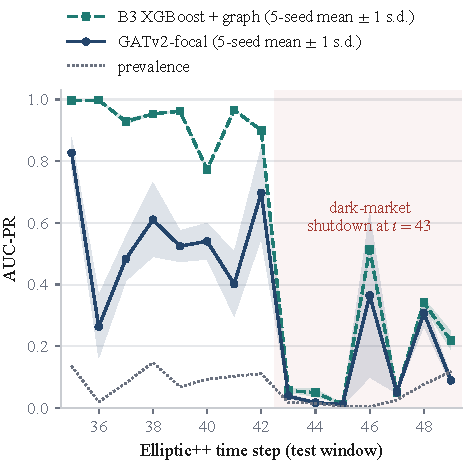
\includegraphics[width=\columnwidth]{figures/fig3_timestep_crater.pdf}
\caption{Per-time-step AUC-PR across the Elliptic++ test window for
GATv2-focal and B3: 5-seed means, with shaded bands of one sample standard
deviation. Both models hold up through step 42 and fall towards the prevalence
floor at step 43, where the market closure lands. A single aggregate figure
hides this.}
\label{fig:crater}
\end{figure}

\begin{table}[t]
\caption{AUC-PR before and after the step-43 market closure (5 seeds, mean
$\pm$ standard deviation). Each window is scored on its own confirmed test
nodes.}
\label{tab:t1b}
\centering
\footnotesize
\setlength{\tabcolsep}{4pt}
\begin{tabular}{lrrll}
\toprule
Steps & $n$ & Prev. & GATv2-focal & B3 \\
\midrule
35--42 & 9,983 & 0.092 & $0.5737 \pm 0.0623$ & $0.9259 \pm 0.0011$ \\
43--49 & 6,687 & 0.025 & $0.0391 \pm 0.0041$ & $0.0567 \pm 0.0034$ \\
\bottomrule
\end{tabular}
\end{table}

The procurement anchor in Table~\ref{tab:t2} keeps the same ordering and
makes the graph model look even worse. R-GCN scores $0.2808 \pm 0.0087$ against
a prevalence of $0.358$: stable across seeds, and below the base rate. This is
not a label or score inversion. The labels map correctly, and the inverted
scores reach $0.43$ to $0.47$ on every seed. The cause is a reversal over time.
The training firms are 87--89\% cartel-linked, against 36\% in test. Among
firms first seen up to 2010, where the R-GCN takes its loss, every usable
structural feature ranks licit firms above cartel firms. Degree, for example,
has a ROC-AUC of $0.38$ for the label there and $0.61$ in test. A model fit on
that window ranks the test firms backwards. Its validation AUC-PR of $0.94$ to
$0.95$ sits just above the validation prevalence of $0.89$, so validation
cannot reveal the problem. Removing the two component-size features, which
shift most between the periods, does not help ($0.2997 \pm 0.0015$).

Our best tree is XGBoost with the publisher's own precomputed screens added, at
$0.4547 \pm 0.0081$. A linear probe on the seven award screens reaches $0.4752$
on the same test firms (Table~\ref{tab:fulllabel}), above every tree. The
uncomfortable headline for this dataset is that the screens tradition
contributes more than the graph model does.

\begin{table}[t]
\caption{Mendeley EU firm-level results (within the case-control sample,
prevalence $0.358$). Lift-style reading applies. Rule and screen rows are
deterministic; tree and R-GCN rows are 5-seed mean $\pm$ standard deviation.
``+screens'' rows add the publisher's own precomputed screen columns to that
baseline's inputs.}
\label{tab:t2}
\centering
\footnotesize
\setlength{\tabcolsep}{4pt}
\begin{tabular}{lll}
\toprule
Model & AUC-PR & P@18 \\
\midrule
B1 rules & 0.3426 (det.) & 0.47 \\
B2 XGBoost & $0.3849 \pm 0.0099$ & $0.22 \pm 0.00$ \\
B3 XGBoost + graph & $0.3749 \pm 0.0092$ & $0.57 \pm 0.06$ \\
B4 screens & 0.3811 (det.) & 0.78 \\
\textbf{B2 + screens} & $\mathbf{0.4547 \pm 0.0081}$ & $0.66 \pm 0.06$ \\
B3 + screens & $0.3509 \pm 0.0058$ & $0.20 \pm 0.03$ \\
B4 + screens & 0.3874 (det.) & 0.50 \\
R-GCN focal & $0.2808 \pm 0.0087$ & $0.07 \pm 0.04$ \\
\bottomrule
\end{tabular}
\end{table}

\subsection{Queue granularity: the unit you score is not the unit you review}
\label{sec:granularity}

Scoring transactions and scoring actors turn out to be different problems, and
the difference shows up in the numbers. On the Elliptic++ actor graph, R-GCN
reaches $0.2473$ AUC-PR against a prevalence of $0.053$, a lift of $4.7\times$,
and the head of its ranking is remarkably dependable: precision@100 of $0.98$,
stable across seeds.
\PENDING{D25: the five-seed actor run supports or replaces this sentence} Roll those node scores up into review groups, though, and
the queue falls apart. The 2,514 actor alerts from the seed-0 model give
precision@50 of $0.08$.

The transaction-level queue, built from the seed-0 calibrated ensemble, runs
the other way. Its 318 communities condense into 254 alerts at precision@50 of
$0.32$, precision@100 of $0.25$ and precision@200 of $0.135$. That is a triage
list an analyst could work, and its top 50 cover 7.9\% of the illicit
population.
Procurement, built from the seed-0 R-GCN, yields 223 alerts from 1,283
communities at precision@18 of $0.33$.

The lesson for practice is that node-level ranking quality and queue-level
precision are not substitutes for one another. Reporting only the first does not show whether the model is useful for real-world triage. We report both.

\subsection{RQ2: unseen markets and planted motifs}
\label{sec:rq2}

\RQ{2} has two parts. The first asks whether a model trained on confirmed
cases beats the base rate in a procurement market it has never seen. The
second asks which planted collusion motifs unsupervised detectors can recover.

\textbf{Transfer to unseen markets.} Fig.~\ref{fig:transfer} and
Table~\ref{tab:t4} give the two procurement transfer matrices. Held-out
prevalences run from $0.29$ to $0.89$ across the Mendeley folds and from
$0.25$ to $0.55$ across the Garc\'ia folds. Lift over the fold's own
prevalence is therefore the only fair comparator.

\begin{figure}[t]
\centering
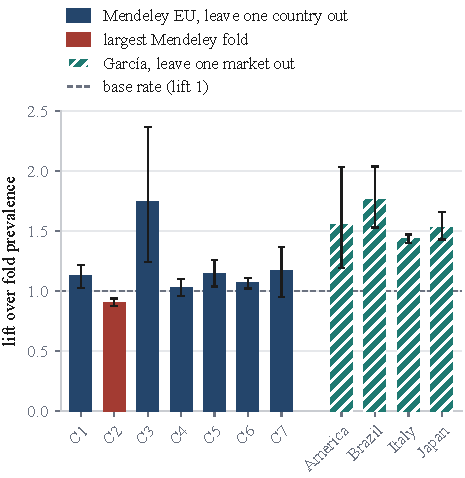
\includegraphics[width=\columnwidth]{figures/fig4_transfer_lift.pdf}
\caption{Transfer lift by held-out fold, with bootstrap 95\% intervals. All
four Garc\'ia markets beat their base rate under leave-one-market-out. On
Mendeley's leave-one-country-out folds (C1--C7, the release's country codes)
the pooled lift is $0.93$, and the largest fold, C2 with 750 of 1,001 firms,
falls below $1.0$. A bar at or below $1.0$ has done no better than the fold's
own base rate.}
\label{fig:transfer}
\end{figure}

\begin{table}[t]
\caption{Procurement transfer matrices, 5 seeds per fold. Lift is AUC-PR
divided by the held-out fold's own prevalence; $1.0$ means no better than the
fold's base rate. Fold AUC-PR is the mean $\pm$ standard deviation over seeds;
brackets give a stratified bootstrap 95\% interval (2,000 resamples) on the
seed-averaged scores. Pooled rows score all held-out firms together (mean
$\pm$ standard deviation over seeds). Size-weighted lift weights each fold by
its $n$.}
\label{tab:t4}
\centering
\footnotesize
\setlength{\tabcolsep}{2pt}
\begin{tabular}{lrrll}
\toprule
Held-out fold & $n$ & Prev. & AUC-PR & Lift [95\% CI] \\
\midrule
\multicolumn{5}{l}{\textit{Mendeley EU --- leave-one-country-out}} \\
\quad country\_1 & 30 & 0.77 & $0.8664 \pm 0.0224$ & 1.13 [1.03, 1.22] \\
\quad country\_2 & 750 & 0.72 & $0.6464 \pm 0.0182$ & 0.90 [0.87, 0.94] \\
\quad country\_3 & 63 & 0.29 & $0.4983 \pm 0.0603$ & 1.74 [1.24, 2.36] \\
\quad country\_4 & 76 & 0.72 & $0.7427 \pm 0.0812$ & 1.03 [0.96, 1.10] \\
\quad country\_5 & 60 & 0.67 & $0.7630 \pm 0.0473$ & 1.14 [1.04, 1.26] \\
\quad country\_6 & 9 & 0.89 & $0.9527 \pm 0.0346$ & 1.07 [1.02, 1.11] \\
\quad country\_7 & 13 & 0.69 & $0.8091 \pm 0.0060$ & 1.17 [0.95, 1.36] \\
\quad Pooled & 1,001 & 0.69 & $0.6404 \pm 0.0153$ & $0.93 \pm 0.02$ \\
\quad Size-weighted & & & & 0.99 \\
\midrule
\multicolumn{5}{l}{\textit{Garc\'ia Rodr\'iguez --- leave-one-market-out}} \\
\quad America & 120 & 0.25 & $0.3894 \pm 0.1080$ & 1.56 [1.19, 2.03] \\
\quad Brazil & 272 & 0.29 & $0.5063 \pm 0.1161$ & 1.77 [1.53, 2.04] \\
\quad Italy & 821 & 0.55 & $0.7858 \pm 0.0585$ & 1.43 [1.40, 1.47] \\
\quad Japan & 1,665 & 0.28 & $0.4295 \pm 0.0223$ & 1.53 [1.43, 1.66] \\
\quad Pooled & 2,878 & 0.36 & $0.4827 \pm 0.0544$ & $1.36 \pm 0.15$ \\
\quad Size-weighted & & & & 1.53 \\
\midrule
\multicolumn{5}{l}{\scriptsize Macro lift (unweighted mean of the fold
lifts): $1.17$ Mendeley, $1.57$ Garc\'ia.} \\
\bottomrule
\end{tabular}
\end{table}

All four Garc\'ia markets beat their own base rate under
leave-one-market-out, and every per-fold 95\% interval for lift lies above 1.
Pooled over all held-out firms, the lift is $1.36 \pm 0.15$ across seeds;
weighted by fold size, it is $1.53$. The Italy fold is strong enough that a
three-alert queue over it returns three confirmed cartels. Mendeley
leave-one-country-out does not behave nearly so well. \texttt{country\_2}
holds 750 of the 1,001 held-out firms and lands at $0.90$ (95\% CI
$[0.87, 0.94]$), below its own base rate. Pooled over all firms, the Mendeley
lift is $0.93 \pm 0.02$; weighted by size, it is $0.99$. Four folds have an
interval above 1, and together they hold 162 firms. The macro lift of $1.17$
therefore comes from small folds. The data release names the seven countries
but does not say which code is which~\cite{mendeley2025}, so the folds keep
their codes.

\textbf{Planted motifs.} Because confirmed cartels are scarce, we plant known
motifs into the unlabelled 163,327-node OCDS Georgia window and measure
recovery at a fixed budget. Only the unsupervised arms can run without labels,
so this experiment measures how detectable each planted motif is, not what a
supervised model learns from it. Table~\ref{tab:t6} shows a clear difference
between the two types of motifs.
\label{sec:injection}

\begin{table}[t]
\caption{Injected-member recall@2000 on the OCDS Georgia window (population
163,327; 5 seeds, mean $\pm$ s.d.; rank-fusion unlabelled mode --- the
unsupervised arms are the only ones available without labels). Note the wide
dispersion on the two recovered families: the seed-to-seed spread is larger
than several of the between-method gaps.}
\label{tab:t6}
\centering
\footnotesize
\setlength{\tabcolsep}{1.5pt}
\begin{tabular}{lllll}
\toprule
Motif family & DOMINANT & Ens.\ (rank) & Floor & GAE \\
\midrule
Coordinated cluster & $0.37 \pm 0.15$ & $\mathbf{0.92 \pm 0.17}$ & $0.12 \pm 0.00$ & $0.91 \pm 0.12$ \\
Common control & $\mathbf{0.58 \pm 0.04}$ & $0.44 \pm 0.02$ & $0.43 \pm 0.00$ & $0.47 \pm 0.02$ \\
Partition & $0.17 \pm 0.01$ & $0.03 \pm 0.03$ & $0.00 \pm 0.00$ & $0.05 \pm 0.01$ \\
Rotation & $0.08 \pm 0.01$ & $0.00 \pm 0.00$ & $0.00 \pm 0.00$ & $0.04 \pm 0.01$ \\
Cover bid & $0.01 \pm 0.01$ & $0.00 \pm 0.00$ & $0.00 \pm 0.00$ & $0.01 \pm 0.01$ \\
\bottomrule
\end{tabular}
\end{table}

Motifs that change the shape of the graph are detected more easily, with coordinated clusters reaching $0.92$ recall and common control reaching $0.58$. Motifs that alter only who wins stay
nearly invisible. Rotation, cover bidding and market partition never exceed
$0.17$ under any method we tried. No amount of tuning will fix this, because the
limitation is structural. Bid rotation leaves the co-bidding topology almost
exactly as it found it and moves only the award labels along the edges.
Catching it calls for award-sequence features, not deeper message passing. We
think this is among the more useful negatives we report, given how often the
cartel literature treats rotation as a flagship detectable pattern.

A caveat belongs with that headline. Coordinated-cluster recall carries a
standard deviation of $0.17$ over five seeds. The apparent ordering between the
rank ensemble at $0.92$ and the graph autoencoder at $0.91$ therefore sits well
inside noise. What the experiment supports is the family-level split between
shape-changing and award-changing motifs. It does not support a ranking of
unsupervised detectors, and we do not offer one.

\subsection{RQ4: cross-domain transfer is asymmetric and needs labels}
\label{sec:rq4}

\textbf{Frozen probes.} We freeze an encoder trained on one domain and probe it
on the other. Neither encoder ever ingests raw features. Both domains enter
through the same ten-column structural template, z-scored within each graph,
so the 183 Elliptic++ columns and the procurement screens never reach an
encoder. Table~\ref{tab:fulllabel} compares each frozen probe at full labels
with probes on the target's own inputs. The two directions disagree. Financial
to procurement reaches $0.2843$ against a prevalence of $0.358$, which is below
the base rate and therefore no signal at all. Procurement to financial reaches
$0.1502$ against $0.065$, a lift of $2.3$. It beats a probe on the target's own
structural template by $0.042$ (95\% CI $[0.026, 0.059]$). A logistic probe on
the inputs of B2 reaches $0.2991$ on the same nodes, however, and B2 itself
reaches $0.8039 \pm 0.0017$. The transferred encoder carries some structural
signal, but far less than the target's own features.

\begin{table}[t]
\caption{Cross-domain probes at full labels, on the published probe's train
and test pools. Each probe is a class-balanced logistic regression: on
embeddings from the stored source encoder (frozen), on the target's own
structural template (structural), or on the inputs of B2 (B2-input). Brackets
give stratified bootstrap 95\% intervals; the B2 row is the 5-seed tree
result.}
\label{tab:fulllabel}
\centering
\footnotesize
\setlength{\tabcolsep}{3pt}
\begin{tabular}{lll}
\toprule
 & Fin.\ $\rightarrow$ proc. & Proc.\ $\rightarrow$ fin. \\
\midrule
Test nodes, prevalence & 363, 0.358 & 16,670, 0.065 \\
Frozen probe & $0.2843$ $[0.268, 0.311]$ & $0.1502$ $[0.135, 0.169]$ \\
Structural probe & $0.2705$ $[0.255, 0.293]$ & $0.1084$ $[0.100, 0.118]$ \\
B2-input probe & $0.4752$ $[0.421, 0.545]$ & $0.2991$ $[0.280, 0.322]$ \\
B2 XGBoost & $0.3849 \pm 0.0099$ & $0.8039 \pm 0.0017$ \\
\bottomrule
\end{tabular}
\end{table}

\textbf{Label efficiency.} Fig.~\ref{fig:labeleff} sweeps how many
target-domain labels are available, with five draws per budget. Below 1,000
labels, ten of the twelve budgets show a negative transfer gain. The two
positive gains, both $+0.002$, lie within one standard deviation of zero. At those budgets the frozen source probe does no better than a probe
trained on the target's own structural features. Procurement to financial
pulls ahead only from 1,000 labels ($+0.013$) and reaches $+0.042$ at full
labels. In the other direction, no probe's mean AUC-PR reaches the base rate
at any budget. Transfer here is a convenience once labels are plentiful, not a
cold-start solution.

\begin{figure}[t]
\centering
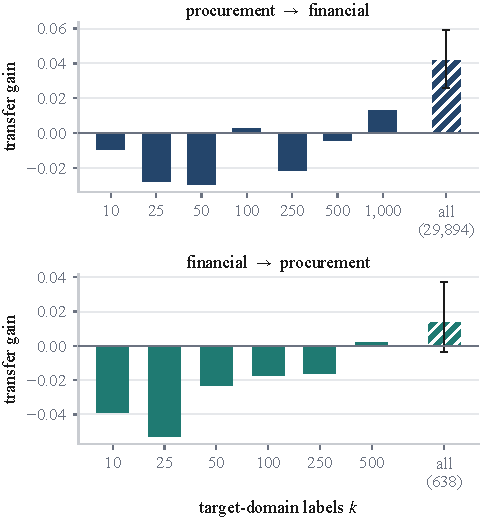
\includegraphics[width=\columnwidth]{figures/fig6_label_efficiency.pdf}
\caption{Cross-domain label efficiency. Each bar gives the gain of a frozen
source-domain probe over a probe trained on the target's own structural
features, at the same label budget (five draws per budget). The hatched bar
uses every training label (Table~\ref{tab:fulllabel}), with its paired
bootstrap 95\% interval. Below 1,000 labels, ten of twelve bars are negative
and the other two lie within one standard deviation of zero. Transfer does not
help the cold-start problem in either direction.}
\label{fig:labeleff}
\end{figure}

\subsection{Robustness, ablations, and a sharp negative}
\label{sec:robustness}

Table~\ref{tab:t7} collects the component ablations, and two conventions govern
how to read it. A ``$-$'' row takes a component out of the adopted model, so its
delta is the cost of removal. A ``$+$'' row adds a variant we evaluated and did
not adopt, so its delta is a rejection margin. These are different measures and should not be compared directly; only the ``$-$'' rows show how much each component affects the model. Each delta is measured against the reference result with the same setup, and we never compare a seed-0 result with a multi-seed mean.

\begin{table}[t]
\caption{Component ablations. ``$-$'' rows are ablation costs; ``$+$'' rows
are rejection margins for variants that were measured and not adopted.}
\label{tab:t7}
\centering
\footnotesize
\setlength{\tabcolsep}{3.5pt}
\begin{tabular}{llll}
\toprule
Arm & Basis & AUC-PR & $\Delta$ \\
\midrule
GATv2-focal (headline) & 5 seeds & $0.4729 \pm 0.0525$ & ref. \\
\quad $-$ focal loss & 5 seeds & $0.4388 \pm 0.0505$ & $-0.0341$ \\
Calibrated ensemble & 5 seeds & $0.4434 \pm 0.0501$ & ref. \\
\quad $-$ unsup.\ members & 5 seeds & $0.4729 \pm 0.0525$ & $+0.0295$ \\
GATv2-focal (headline) & seed 0 & $0.5492$ & ref. \\
\quad $-$ bidir.\ edges & seed 0 & $0.3549$ & $\mathbf{-0.1943}$ \\
\quad $+$ structural chan. & seed 0 & $0.3781$ & $-0.1711$ \\
\quad $+$ line-graph chan. & seed 0 & $0.4986$ & $-0.0506$ \\
\quad $+$ context fusion & seed 0 & $0.3242$ & $-0.2250$ \\
Mendeley B2 XGBoost & 5 seeds & $0.3849 \pm 0.0099$ & ref. \\
\quad $+$ dataset screens & 5 seeds & $0.4547 \pm 0.0081$ & $+0.0698$ \\
\bottomrule
\end{tabular}
\end{table}

Direction-awareness is the component that makes the biggest difference. Dropping reverse edges reduces AUC-PR by $0.194$. This is in line with the gains Egressy et al.\ report from reverse message passing~\cite{egressy2024}, on a different dataset and by a different team. Focal loss gives a smaller improvement of $0.034$. Extra input channels reduced performance every time we tried them: the structural, line-graph and context-fusion variants all performed worse than using the raw features alone.
We see this as an interaction between model capacity and distribution shift, not as evidence that these channels carry no information in general.


\textbf{Protocol sensitivity, and where it is not flat.} We swept the Jaccard
suppression threshold over $\{0.3, 0.4, 0.5, 0.6, 0.7\}$ crossed with three
hit-rule settings. The two axes give different results, so we do not combine them into one robustness claim.

Suppression does not change the alert set. At every threshold, the financial queue keeps all 254 alerts and the procurement queue keeps all 223, with none suppressed anywhere in the grid. The communities barely overlap, so non-maximum suppression does not affect the results. This means the published queues are not dependent on a tuned de-duplication setting.

The hit rule is different. Our published queue counts a group as a hit when at least one member is confirmed. If we instead require $0.1$ of the members to be confirmed, financial precision@50 falls from
$0.32$ to $0.30$. P@100 falls from $0.25$ to $0.23$, and P@200 from $0.135$ to
$0.125$. Tightening further to $0.25$ costs nothing beyond that. Procurement
stays flat on both axes, with P@18 remaining at $0.33$ throughout. So about $0.02$ of
our headline queue precision rests on a definitional choice. We report the
looser rule and state the dependence, since presenting the number as though no
choice were involved would not be true.

\textbf{The label-noise result.} Fig.~\ref{fig:noise} carries the sharpest
negative in the paper. We flipped a fraction of the training labels at random
and tracked validation and test AUC-PR together. Test performance climbed
steadily, from $0.4827 \pm 0.0616$ on clean labels to $0.5978 \pm 0.0248$ with
20\% flipped. Validation fell over the same range, $0.9418$ down to $0.5692$.
The curves move apart.

\begin{figure}[t]
\centering
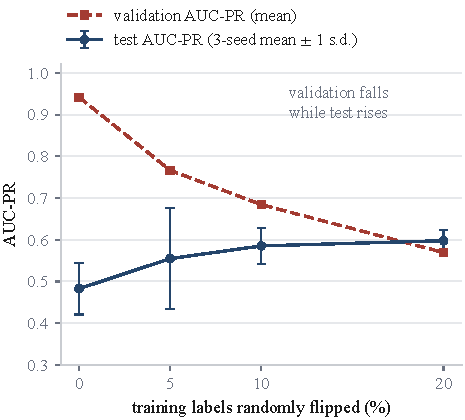
\includegraphics[width=\columnwidth]{figures/fig5_label_noise.pdf}
\caption{Label-noise robustness on Elliptic++ (GATv2-focal, 3 seeds per rate).
Corrupting training labels \emph{improves} test AUC-PR while validation
collapses. Model selection on validation is optimising against the wrong
curve.}
\label{fig:noise}
\end{figure}

A plausible explanation is that validation (steps 30--34) sits entirely in the
pre-shift regime, while test straddles the step-43 break. Label noise may act
as a regulariser that stops the model committing too hard to pre-shift
structure. That costs validation and buys test.
\PENDING{B7: whether explicit regularisers do the same, and which measurements support the claim}

This is a diagnostic, not a training recommendation. It shows that validation
selection is unreliable under this shift.

\textbf{AMLworld at scale.} For completeness we report a negative at 5M edges:
tree baselines score $0.0063$ (B2) and $0.0062$ (B3) against an account-level
prevalence of $0.0103$ (Section~\ref{sec:prevalence}), which puts both below
chance. Their inverted scores reach $0.0211$ and $0.0239$, about twice the
prevalence. The labels map correctly, so this is not an inversion bug. The
cause is the split. Accounts are heavily front-loaded, so a node-first-seen
split puts the training cut one hour into the data, and training features see
only 344,747 of 5,078,345 transactions. In that hour the money-flow features
carry almost no label signal (ROC-AUC $0.49$ to $0.54$). Over the full window
the same features carry a strong one (up to $0.74$). The trees
therefore learn from noise, and their splits do not carry over to accounts
observed for ten days. We use AMLworld for what it was designed to do,
injection against known ground truth, and not as a supervised benchmark.

% =====================================================================
\section{Explanation Study}
\label{sec:rq3}
% =====================================================================

\RQ{3} asks how faithful the subgraph explanations are and how many alerts
match a red-flag pattern that practitioners already use. We answer it from
fidelity and coverage measurements on the published queue. The answer is
mixed. PGExplainer's explanations pass PyG's fidelity sanity check on 49 of 50
alerts. Under a stricter uniform test only 25 of 50 pass, and no explainer
produces sparse explanations. On the financial queue, 15 of 50 alerts match a
red-flag pattern; on the procurement queues none do.

\textbf{Choosing an attribution method.} We ran a three-arm ablation over the
top members of the 50 highest-ranked financial alerts, comparing GNNExplainer,
PGExplainer and raw attention (Table~\ref{tab:explainers}). Each arm keeps the
20 highest-scoring edges of a two-hop window around the node. Under PyG's
fidelity measure~\cite{fey2019}, PGExplainer returned sane attributions on 49 of the 50 nodes,
where GNNExplainer managed 10, and it took under a third of the time. We
adopted it. Its bundles carry an implausible-fidelity flag on 1 of 50 alerts,
against 40 of 50 for GNNExplainer.

A uniform test gives a less flattering picture. We remove or keep the chosen
edges outright and measure the change in the model's probability for its own
prediction. Following the standard definitions~\cite{yuan2023,agarwal2023},
Fidelity+ is the drop when the explanation is removed; Fidelity$-$ is the drop
when only the explanation is kept. Under this test the three arms
are close. Fidelity+ ranges from $0.049$ to $0.052$, and 22 to 25 of the 50
explanations of each arm pass (Fidelity+ $\geq$ Fidelity$-$). Sparsity is low
because most two-hop windows hold few more edges than the 20 kept, and
attention keeps almost every edge. The arms also largely agree on which edges
matter: the mean Jaccard overlap of their edge sets runs from $0.65$ to $0.88$.
Attention, popular because it looks like interpretability for
free~\cite{jain2019}, matches GNNExplainer under this test.

\begin{table}[t]
\caption{Explainer metrics on the top members of the 50 highest-ranked
financial alerts (seed-0 GATv2, two-hop windows, 20 kept edges). ``PyG sane''
uses PyG's fidelity measure. Hard-mask Fidelity$\pm$ are mean probability
drops for the model's own prediction; ``hard sane'' counts nodes with
Fidelity+ $\geq$ Fidelity$-$. Sparsity is the share of window edges left out.
Time is wall-clock on one 4-core laptop CPU.}
\label{tab:explainers}
\centering
\footnotesize
\setlength{\tabcolsep}{2.5pt}
\begin{tabular}{lrrrrrr}
\toprule
Arm & PyG sane & Fid+ & Fid$-$ & Hard sane & Sparsity & Time (s) \\
\midrule
PGExplainer & 49/50 & 0.052 & $-0.006$ & 25/50 & 0.12 & 18.1 \\
GNNExplainer & 10/50 & 0.049 & 0.000 & 22/50 & 0.29 & 57.8 \\
Attention & --- & 0.049 & 0.000 & 22/50 & 0.01 & 0.6 \\
\bottomrule
\end{tabular}
\end{table}

\textbf{Motif matching and red-flag mapping.} A rule-based matcher emitting
nine motif types (cycle, fan-in, fan-out, pass-through, common control,
rotation, cover bid, partition, clique) runs over every alert's subgraph. It is
implemented independently of the injection generators, so the two
cross-validate each other. A parameterised test asserts that it recovers all
ten generator families, five financial and five procurement, at 100\% recall
on fixtures.
Coverage on real queues is patchier. On the financial queue 15 of 50 bundles
carry a proven motif with FATF citations attached, and on the actor queue 15 of
20. On the procurement queues the count is zero. The Mendeley alert communities
and the three Garc\'ia Italy alerts are simply too small, often just two firms,
to contain a shape the matcher can prove. That is a coverage limitation and we
would rather record it than paper over it with a weaker claim.

\textbf{Copilot gate.} The release gate checks 26 golden cases against two separate requirements. The first has zero tolerance and applies to the released output: no guilt-attributing language can be released, and a deterministic guard enforces this instead of relying on a prompt. The second requires a grounding score of $0.9$, meaning every number quoted by the assistant must appear in the rows it actually read. The gate passes. Grounding is 24 of 26 cases ($0.923$; Wilson 95\% CI~\cite{wilson1927} $[0.759, 0.979]$). Released guilt violations are at zero, and draft rewrites have 1 of 26 cases against a $10\%$ ceiling. The interval is wide: with 26 cases, its lower bound sits below the $0.9$ threshold, so the gate cannot show that grounding exceeds it.

We report the two grounding misses instead of hiding them through rounding because they are not random. Both are the newest cases in the set, and both use the tool we added most recently, the injection-study reader. One quoted a recall figure that was not present in the rows it had retrieved; the other left out an expected motif name from an answer that was otherwise well grounded. Growing the golden set from 24 to 26 left the older cases untouched but exposed problems in the new ones. For a bounded agent whose tool surface has just been expanded, this is a useful failure to find. It also shows why the golden set should be extended whenever a new tool is added instead of relying on a previously perfect score.

Two earlier failures were fixed with prompt rules and did not need model changes. The agent once repeated a question presuming guilt in its own words while denying the premise. In another case, it changed a metric from  $0.32$ to ``32\%'' in a way that broke traceability back to the artifact. The deterministic guard, rather than the model simply following instructions, is what keeps the released-output bar at zero.

\textbf{Practitioner phase.} The instrument, the rater packets and the scoring
rubric are built and released. \textbf{The human study has not been run.} We
therefore answer \RQ{3} from fidelity and coverage measurements, not from
practitioner judgement, and record the missing study as a limitation. Using our
own judgement in place of practitioners' would defeat the purpose of the
study. The released protocol specifies a fallback panel of rubric-trained
graduate raters, including at least one domain expert.

% =====================================================================
\section{Regulatory Alignment and Ethics}
\label{sec:regulatory}
% =====================================================================

We use the EU AI Act's requirements for high-risk AI systems as a design
standard. They cover technical documentation, automatic logging, transparency
towards deployers and human oversight~\cite[Arts.~11--14]{aiact}. Since the
Digital Omnibus on AI entered into force on 27~July 2026, these requirements
apply to stand-alone Annex~III systems from 2~December 2027~\cite{omnibus}.
We do not claim that this screener is a high-risk system. Annex~III
point~5(b) covers AI systems that evaluate the creditworthiness of natural
persons or establish their credit score, except systems used to detect
financial fraud~\cite{aiact}. The Commission's draft guidelines state that
anti-money-laundering and counter-terrorist-financing systems are not covered
by that fraud exception. They add that such systems are out of scope where
they do not assess creditworthiness~\cite[para.~309]{eccguidance}. The draft
was published on 19~May 2026 for consultation, which closed on 23~July 2026.
It is not binding, and its final wording may differ.

In the UAE, Article~149 of Federal Decree-Law No.~6 of 2025 requires licensed
financial institutions to implement robust fraud prevention and detection
mechanisms~\cite{uaefdl2025}. It also lets the Central Bank require data on
fraud patterns, and it requires cooperation with the Central Bank's fraud
investigations. On the procurement side, public procurement accounted for
12.7\% of GDP across OECD countries in 2023~\cite[p.~146]{oecdgaag2025}. The
OECD's 2025 guidelines give procurement officials checklists for designing
tenders against collusion and for spotting red flags~\cite{oecd2025}.

We map each requirement onto something the system actually does.
Every alert ships with a subgraph, a matched motif and a red-flag citation,
which is the interpretability requirement made concrete. The queue stops at a
fixed budget, so the system is built as a triage instrument for a human reviewer
and could not act autonomously even if asked. Artifacts are immutable files and
the serving layer is read-only, so an auditor can reconstruct exactly what an
analyst saw. The caveat attaches at the API boundary where no client can
suppress it, and a release gate, not a prompt convention, enforces the
guilt-language guard.

\textbf{Scope boundary.} This system determines no legal guilt. It ranks cases
for human investigation. We target the maturity of a validated prototype, TRL
3--4, on public and synthetic data, and we used no personal or classified data
at any point. We say so in the paper for the same reason the system says so on
every response. Misreading a screening score as an accusation does real harm, and
the language guarding against that is part of the design.

% =====================================================================
\section{Limitations}
% =====================================================================

\begin{itemize}
\item \textbf{The Elliptic shift has a strong effect on the financial results}, and validation selection cannot detect it \PENDING{B7: the measurements that support this}. Test numbers on this benchmark should therefore be read as dependent on the regime.
\item \textbf{Anonymised features limit what an explanation can say.} Elliptic’s features contain no names, so financial explanations remain structural. Amount-level explanations are only available on AMLworld, which is synthetic.
\item \textbf{Mendeley is case-control.} Lift is the appropriate comparator instead of raw AUC-PR, and it says nothing about population-level precision.
\item \textbf{Garc\'ia identity coverage reaches four of six markets}, so the co-bidding identity graphs do not cover the whole benchmark.
\item \textbf{Award-pattern motifs recover badly} especially rotation, cover bidding and partition. This limits what we can claim about the procurement side specifically.
\item \textbf{The copilot's grounding is imperfect and depends on its tool
surface.} Grounding stands at $0.923$ on the current 26-case gate, with both misses occurring on the tool we added last. The released-output guarantee is deterministic and has zero violations, but grounding is a statistical measure and may drop when the agent gains new tools faster than the golden set grows.
\item \textbf{The practitioner study's human phase has not been run}, so
\RQ{3} currently relies on fidelity and coverage measurements rather than practitioner judgement.
\item \textbf{Compute envelope.} Everything published here ran on CPU,
full-batch. Neighbour-sampled minibatch training on the five-million-edge
AMLworld graph, and the PNA and GIN comparisons that would depend on it, sit
outside that envelope.
\end{itemize}

% =====================================================================
\section{Reproducibility}
\label{sec:reproducibility}
% =====================================================================

One YAML file equals one experiment, and every experimental result in this
paper traces to a committed config. The one exception is the machine-class
difference quoted below, which comes from the project ledger. A number manifest
records the artifact behind each printed value, and an audit script checks
every value against it. Two repository tests guard the number-to-config map.
One fails continuous integration if Appendix~\ref{app:repro} names a
configuration that does not exist. The other keeps the full map in the
repository documentation in step with the configuration directory in both
directions.
Alongside it go pinned dependencies and a Python version, per-dataset checksum
manifests recording licences, five datasheets~\cite{gebru2021}, a model
card~\cite{mitchell2019}, and every table
here as a regeneration target. We verified byte-level cross-machine
reproducibility for the tree baselines, the leave-one-country-out fold and the
leave-one-market-out matrix. With the stored encoder weights, the
procurement-to-financial probe also reproduces exactly. The
financial-to-procurement probe gives $0.2841$ on the original machine and
$0.2843$ on a second one. Torch GNN training is deterministic on one machine,
and its results depend on the machine class. A second machine of the same
class reproduced the seed-0 GATv2 run bit for bit; one of another class
differed by about $0.02$. Seed variance of about $\pm 0.05$ swamps that
difference. A dedicated suite enforces the leakage
guarantees and runs as its own continuous-integration step. The full suite comes
to 425 tests.

% =====================================================================
\section{Conclusion}
% =====================================================================

One stack does serve both ledgers, and building it that way is what made the
negative results legible. Under a strict protocol, gradient-boosted trees on
graph features still beat the graph neural networks on the financial anchor.
The whole gap lies before the step-43 market closure, which defeats both model
families.
Calibrated fusion is necessary once members are fused, but it did not beat its
best member. Transfer between procurement markets holds on Garc\'ia, with a
pooled lift of $1.36$. It does not hold on Mendeley, where the pooled lift is
$0.93$ and the largest market falls below its base rate. Across domains, a frozen
procurement encoder carries some structural signal into the financial domain.
A probe on the target's own features doubles it, and the reverse direction
gives no signal. Below 1,000 labels, transfer never clearly helps.
Corrupting training labels lifts test performance while validation falls away,
so validation selection is unreliable under this shift.
\PENDING{B7: comparison with explicit regularisers}

Several of these findings would be hidden by a single-seed,
validation-selected, aggregate-only evaluation: the spread across seeds, the
failing largest market and the validation blind spot. That is what we mean by
calling the protocol a contribution. Alongside it we ship a screening
instrument. It ranks groups for a human at a fixed budget, explains each flag
in the reviewer's own red-flag vocabulary, and cannot call anyone guilty.

\textbf{Future work.} One beneficial owner may control both a bid-rigging firm
and the accounts that launder its proceeds. A natural next step is to test
whether a joint model with shared-control edges finds such dual actors better
than two separate detectors.

\section*{Acknowledgements}

[Placeholder --- funding, compute, and dataset-provider acknowledgements to be
completed before submission.]

\appendices

\section{Number-to-Config Map}
\label{app:repro}

Table~\ref{tab:repro} ties every headline number in this paper to the one
committed configuration that produces it. A repository hygiene test fails
continuous integration if the table names a configuration that does not exist,
and a second test keeps the repository's full map in step with the
configuration directory in both directions. Run any row as
\texttt{collusiongraph <verb> -c configs/experiment/<config>}. Outputs land in a
gitignored results directory and are never committed.

\begin{table*}[t]
\caption{Published number $\rightarrow$ config. Multi-seed rows run seeds 0--4
and are resumable; completed seeds are never retrained.}
\label{tab:repro}
\centering
\footnotesize
\setlength{\tabcolsep}{4pt}
\begin{tabular}{p{0.40\textwidth}p{0.54\textwidth}}
\toprule
Config (\texttt{configs/experiment/}) & Produces \\
\midrule
\texttt{baselines\_elliptic\_pp} & B1 rules, $0.0576$ (Table~\ref{tab:t1}) \\
\texttt{baselines\_elliptic\_pp\_} \texttt{multiseed} & B2 $0.8039$, B3 $0.8123$, per-step AUC-PR \\
\texttt{baselines\_elliptic\_pp\_} \texttt{local\_multiseed} & B2-local $0.7879$, B3-local $0.7959$ \\
\texttt{gnn\_elliptic\_pp\_gatv2\_} \texttt{focal\_multiseed} & the headline GNN number, $0.4729 \pm 0.0525$ \\
\texttt{significance\_elliptic\_pp\_} \texttt{multiseed} & Table~\ref{tab:t3} \\
\texttt{derived\_numbers} & Table~\ref{tab:t1b}; copilot Wilson interval; probe lift \\
\texttt{baselines\_elliptic\_pp\_} \texttt{calib\_multiseed} & B3 trained on steps 1--29, $0.8012$ \\
\texttt{fusion\_gatv2\_b3\_} \texttt{multiseed} & GATv2 + B3 calibrated fusion, $0.7760$ \\
\texttt{gnn\_elliptic\_pp\_gatv2\_} \texttt{wce\_multiseed} & $-$focal ablation, $0.4388 \pm 0.0505$ \\
\texttt{gnn\_elliptic\_pp\_gatv2\_} \texttt{focal\_unidir} & $-$bidirectional edges, $0.3549$ \\
\texttt{gnn\_elliptic\_pp\_gatv2\_} \texttt{focal\_multi} & $+$structural channel, $0.3781$ \\
\texttt{gnn\_elliptic\_pp\_gatv2\_} \texttt{focal\_line} & $+$line-graph channel, $0.4986$ \\
\texttt{gnn\_elliptic\_pp\_gatv2\_} \texttt{focal\_cf} & $+$context fusion, $0.3242$ \\
\texttt{ensemble\_elliptic\_pp\_} \texttt{multiseed} & calibrated $0.4434 \pm 0.0501$ vs.\ rank $0.0511 \pm 0.0019$ \\
\texttt{alert\_queue\_elliptic\_pp\_} \texttt{ensemble} & the financial queue: 254 alerts, P@50 $0.32$ \\
\texttt{sensitivity\_elliptic\_pp} & financial NMS and hit-rule grid \\
\texttt{label\_noise\_elliptic\_pp} & the noise curve, $0.4827 \rightarrow 0.5978$ \\
\texttt{explainer\_metrics\_} \texttt{elliptic\_pp} & Table~\ref{tab:explainers} \\
\texttt{explanations\_elliptic\_pp} & financial bundles, 15 of 50 with a motif \\
\texttt{gnn\_elliptic\_actor\_rgcn} & the actor-graph R-GCN \\
\texttt{alert\_queue\_elliptic\_actor} & the actor queue \\
\texttt{explanations\_elliptic\_actor} & actor bundles \\
\texttt{baselines\_mendeley\_eu} & B1 $0.3426$ / B4 $0.3811$ \\
\texttt{baselines\_mendeley\_eu\_} \texttt{multiseed} & B2 $0.3849$ / B3 $0.3749$ \\
\texttt{baselines\_mendeley\_} \texttt{screens\_ablation\_} \texttt{multiseed} & B2+screens $0.4547$, B3+screens $0.3509$ \\
\texttt{baselines\_mendeley\_b4\_} \texttt{precomputed} & B4 + screens $0.3874$ \\
\texttt{gnn\_mendeley\_rgcn\_} \texttt{multiseed} & R-GCN, $0.2808 \pm 0.0087$ \\
\texttt{gnn\_mendeley\_rgcn\_} \texttt{nocomm\_multiseed} & R-GCN without component features, $0.2997$ \\
\texttt{diagnose\_below\_chance} & the below-chance diagnoses \\
\texttt{alert\_queue\_mendeley\_eu} & the procurement queue: 223 alerts, P@4 $0.50$ \\
\texttt{sensitivity\_mendeley\_eu} & procurement NMS and hit-rule grid \\
\texttt{explanations\_mendeley\_eu} & procurement bundles, 0 of 20 with a motif \\
\texttt{transfer\_loco\_matrix\_} \texttt{mendeley} & 7-fold LOCO (Table~\ref{tab:t4}) \\
\texttt{transfer\_lomo\_matrix\_} \texttt{garcia} & 4-market LOMO (Table~\ref{tab:t4}) \\
\texttt{transfer\_pooled\_lift} & pooled lift $0.93$ / $1.36$, fold intervals \\
\texttt{cross\_domain\_full\_} \texttt{label\_comparison} & Table~\ref{tab:fulllabel} \\
\texttt{cross\_domain\_probe\_} \texttt{proc2fin} & the procurement source encoder; $0.1502$ \\
\texttt{cross\_domain\_probe\_} \texttt{fin2proc} & the financial source encoder; $0.2841$ on the original machine \\
\texttt{label\_efficiency\_*} & both label-efficiency curves \\
\texttt{injection\_recovery\_ocds\_} \texttt{georgia\_multiseed} & Table~\ref{tab:t6}; coordinated cluster $0.92 \pm 0.17$ \\
\texttt{baselines\_amlworld} & the 5M-edge negative, $0.0063$ / $0.0062$ \\
\texttt{practitioner\_study} & rater packets and manifest \\
\bottomrule
\end{tabular}
\end{table*}

\section{Protocol Guarantees}

A dedicated leakage test, not a convention, enforces each of the following:
strict-inductive temporal splits, as-of feature computation,
leave-one-country and leave-one-market entity isolation, and the alert-unit
rules. That suite runs standalone and also as its own continuous-integration
step on every push. A change that lets leakage back in therefore breaks the
build instead of quietly improving somebody's number. Torch GNN training is
deterministic on one machine, and its results depend on the machine class
(Section~\ref{sec:reproducibility}). Seed variance of about $\pm 0.05$
dominates the machine difference, which is why every learned number here
appears as a multi-seed mean with its standard deviation.

\section{Experimental Details}
\label{app:methods}

This appendix gives every setting needed to judge fairness without the
repository. Each value was read from the committed configs and code.

\textbf{Splits.} Elliptic++ is split by time step. The training graph holds
steps 1--34. The loss uses the confirmed nodes of steps 1--29, and early
stopping uses validation AUC-PR on the confirmed nodes of steps 30--34, so
validation is temporal and never a random sample of training nodes. The test
window is steps 35--49. Mendeley is split by the year a firm first appears:
training holds firms first seen up to 2013, and the test set holds the 363
confirmed firms first seen from 2014. The R-GCN takes its loss on firms first
seen up to 2010 and validates on 2011--2013; the trees train on all firms up
to 2013. A firm counts as cartel-linked once it holds an award the release
marks as cartel. Training labels use only awards dated up to the cut, so later
findings cannot leak into training targets; test labels use the full record.
AMLworld splits accounts by first appearance, with the post-window tail
removed. Leave-one-country-out (Mendeley) and leave-one-market-out (Garc\'ia)
hold out one country or market at a time and score it on its own subgraph.
Early stopping uses the smallest other group with at least three confirmed
firms per class: \texttt{country\_7} validates every Mendeley fold except its
own, which \texttt{country\_1} validates, and America validates every
Garc\'ia fold except its own, which Brazil validates. Each fold runs five
seeds.

\textbf{Features.} Elliptic++ carries 183 node columns: the time step, 93
local features, 72 one-hop aggregates and 17 Elliptic++ additions, which
include in- and out-degree and BTC amounts. B2 uses all 183 columns and a
money-flow pack computed from the transaction edges (counts and timing; the
Elliptic++ edges carry no amounts). B2-local keeps the time step and the 93
local features only. On Mendeley, B2 uses the award screens of B4. B3 adds two
groups to B2's inputs. The first is a structural template: in-, out- and
total degree, mutual-dyad degree, clustering, k-core, triangles, burstiness,
the size of the node's connected component, and its degree relative to that
component. The second is the mean of each column over a node's neighbours (the
raw columns on Elliptic++, the structural template on Mendeley). The
``+screens'' rows add the publisher's precomputed screens: the mean and
minimum bids per lot and the mean relative value. Every feature derived from
history is computed as of the training cut for training nodes and on the full
graph for test nodes.

\textbf{Rule and screen baselines.} B1 scores a node by the share of rules it
triggers. Each threshold is a percentile fitted on training nodes only.
Elliptic++ uses five rules: in-degree and out-degree above their 99th
percentiles, velocity above its 95th, median holding time below its 5th, and
mutual-dyad degree above its 99th. Mendeley uses three: number of awards,
market share and buyer concentration, each above its 95th percentile. B4
averages direction-adjusted z-scores of its screens.

\textbf{Models and training.} Table~\ref{tab:hparams} lists the network
settings. Every graph network trains full batch on the CPU with Adam and
weight decay $5 \times 10^{-4}$. The loss is focal with $\gamma = 2$ and no
$\alpha$ weighting; weighted cross-entropy is the ablation arm. Training stops
early on validation AUC-PR, and the best validation epoch is kept. XGBoost
uses 400 trees of depth 6, learning rate 0.1, the histogram method, and a
positive-class weight equal to the ratio of negatives to positives. Its
five-seed rows subsample rows and columns at 0.8.

\begin{table}[h]
\caption{Network settings. Every network uses two layers, Adam and weight decay
$5 \times 10^{-4}$; GATv2 uses four attention heads. ``Folds'' are the LOCO
and LOMO folds; ``probe'' rows are the cross-domain source encoders. ``Pat.''
is the early-stopping patience in epochs.}
\label{tab:hparams}
\centering
\footnotesize
\setlength{\tabcolsep}{3pt}
\begin{tabular}{lrrrrr}
\toprule
Model (data) & Hidden & Dropout & LR & Epochs & Pat. \\
\midrule
GATv2 (Elliptic++) & 64 & 0.3 & 0.005 & 200 & 20 \\
R-GCN (Mendeley, folds) & 64 & 0.3 & 0.01 & 300 & 30 \\
R-GCN (actor graph) & 64 & 0.3 & 0.005 & 120 & 15 \\
SAGE probe (Elliptic++) & 64 & 0.3 & 0.005 & 200 & 20 \\
SAGE probe (Mendeley) & 64 & 0.3 & 0.01 & 300 & 30 \\
DOMINANT, GAE & 32 & --- & --- & 50 & --- \\
\bottomrule
\end{tabular}
\end{table}

\textbf{Tuning.} No model received a hyperparameter search. The trees run
standard settings, and the graph networks run fixed, hand-chosen settings with
early stopping. The tuning budgets are therefore equal, at zero. Because the
trees win every comparison they enter, no positive claim rests on beating an
under-tuned baseline.

\textbf{Unlabelled nodes.} Unlabelled nodes (77\% of Elliptic++
transactions) carry structure in message passing but never enter a loss.
Every metric uses confirmed nodes only. In a queue, an unlabelled member counts
neither towards a hit nor towards a group's confirmed members, and a hit needs
at least one confirmed illicit member.

\textbf{Fusion.} The fused members are GATv2, the only supervised member,
DOMINANT, GAE and the structural floor. Each member is isotonic-calibrated on
the confirmed nodes of steps 30--34, and the fused score is the equal-weight
mean of the calibrated scores. Rank fusion averages rank percentiles. The
GATv2 and B3 fusion trains B3 on steps 1--29, so that steps 30--34 can
calibrate it.

\textbf{Alert queue.} Leiden runs at resolution 1.0 (seed 0) on the
test-window subgraph, and single-node communities are dropped. A group's score
is the mean of its highest calibrated member score and the mean score of its
top quarter of members. Groups above 100 members are excluded (64 on
Elliptic++), and Jaccard non-maximum suppression runs at 0.5. The financial
budgets are 50, 100 and 200 groups: a review capacity of 100, with one step
either side. The procurement budgets are 4, 18 and 36, the top 1, 5 and 10\%
of the 363 test firms.

\textbf{Cross-domain probe.} Each source encoder is a two-layer GraphSAGE
trained on its own domain's structural template. No encoder sees raw features,
so the 183 Elliptic++ columns and the procurement screens never meet an
encoder. Each graph is z-scored with statistics from its own training period.
The frozen encoder embeds the target graph, and a class-balanced logistic
regression (L-BFGS, at most 2,000 iterations) is fitted on the target's
training-period nodes and scored on its test period.

\textbf{Copilot.} The agent uses \texttt{nvidia/nemotron-3-super-120b-a12b}
through NVIDIA NIM at temperature 0, with at most 4,096 tokens per call, and
\texttt{nvidia/nemotron-3-nano-30b-a3b} as a validator. Its prompts live in
\texttt{backend/copilot/agent.py}. The 26 golden cases cover SQL questions
(8), retrieval (4), explanation bundles (3), guardrails (3), honesty (3),
metrics (2), the stress test (2) and alert tools (1). The gate result in
Section~\ref{sec:rq3} comes from a run on 19 August 2026.

\textbf{Compute.} Every run used the CPU and full-batch training, on two
laptops with 11th-generation Intel Core processors (i7-1195G7 and i5-11300H;
4 cores, 8 threads, 16 GB of memory). One GATv2 run takes 14 to 38 minutes,
depending on machine load. The five-seed trees take about six minutes on
Elliptic++ and under a minute on Mendeley, and a Mendeley R-GCN seed takes a
few seconds.

\textbf{Code and data availability.} \PENDING{L3: repository URL and
availability wording, an author decision} The datasets are public and are
downloaded from their canonical sources (Table~\ref{tab:data}). No raw or
modified data is redistributed.

\balance

\begin{thebibliography}{00}
\bibitem{lannoo2021} K. Lannoo and R. Parlour, ``Anti-money laundering in the EU: Time to get serious,'' CEPS-ECRI Task Force Report, Centre for European Policy Studies, Brussels, Belgium, Jan. 2021.
\bibitem{oecd2025} OECD, \emph{OECD Guidelines for Fighting Bid Rigging in Public Procurement (2025 Update)}. Paris, France: OECD Publishing, 2025, doi:10.1787/cbe05a56-en.
\bibitem{aiact} ``Regulation (EU) 2024/1689 of the European Parliament and of the Council of 13 June 2024 laying down harmonised rules on artificial intelligence (Artificial Intelligence Act),'' \emph{Official Journal of the European Union}, L series, 12 Jul. 2024.
\bibitem{omnibus} ``Regulation (EU) 2026/1744 of the European Parliament and of the Council of 8 July 2026 amending Regulations (EU) 2024/1689, (EU) 2018/1139 and (EU) 2023/1230 as regards the simplification of the implementation of harmonised rules on artificial intelligence (Digital Omnibus on AI),'' \emph{Official Journal of the European Union}, L series, 24 Jul. 2026.
\bibitem{eccguidance} European Commission, ``Draft Commission guidelines on the classification of high-risk AI systems,'' draft for targeted stakeholder consultation, 19 May 2026 (consultation closed 23 Jul. 2026; not binding). [Online]. Available: \url{https://digital-strategy.ec.europa.eu/en/library/draft-commission-guidelines-classification-high-risk-ai-systems}
\bibitem{ma2023} X. Ma, J. Wu, S. Xue, J. Yang, C. Zhou, Q. Z. Sheng, H. Xiong, and L. Akoglu, ``A comprehensive survey on graph anomaly detection with deep learning,'' \emph{IEEE Trans. Knowl. Data Eng.}, vol.~35, no.~12, pp.~12012--12038, 2023, doi:10.1109/TKDE.2021.3118815.
\bibitem{gadbench} J. Tang, F. Hua, Z. Gao, P. Zhao, and J. Li, ``GADBench: Revisiting and benchmarking supervised graph anomaly detection,'' in \emph{Adv. Neural Inf. Process. Syst.}, vol.~36, 2023, pp.~29628--29653, doi:10.52202/075280-1289.
\bibitem{liu2022bond} K. Liu \emph{et al.}, ``BOND: Benchmarking unsupervised outlier node detection on static attributed graphs,'' in \emph{Adv. Neural Inf. Process. Syst.}, vol.~35, 2022, pp.~27021--27035, doi:10.52202/068431-1959.
\bibitem{motie2024} S. Motie and B. Raahemi, ``Financial fraud detection using graph neural networks: A systematic review,'' \emph{Expert Syst. Appl.}, vol.~240, art.~122156, 2024, doi:10.1016/j.eswa.2023.122156.
\bibitem{linemv2025} C.-H. Poon, J. Kwok, C. Chow, and J.-H. Choi, ``LineMVGNN: Anti-money laundering with line-graph-assisted multi-view graph neural networks,'' \emph{AI}, vol.~6, no.~4, art.~69, 2025, doi:10.3390/ai6040069.
\bibitem{weber2019} M. Weber, G. Domeniconi, J. Chen, D. K. I. Weidele, C. Bellei, T. Robinson, and C. E. Leiserson, ``Anti-money laundering in Bitcoin: Experimenting with graph convolutional networks for financial forensics,'' presented at the KDD Workshop on Anomaly Detection in Finance, Anchorage, AK, USA, 2019, arXiv:1908.02591.
\bibitem{cardoso2022} M. Cardoso, P. Saleiro, and P. Bizarro, ``LaundroGraph: Self-supervised graph representation learning for anti-money laundering,'' in \emph{Proc. 3rd ACM Int. Conf. AI in Finance (ICAIF)}, 2022, pp.~130--138, doi:10.1145/3533271.3561727.
\bibitem{egressy2024} B. Egressy, L. von Niederh\"ausern, J. Blanu\v{s}a, E. Altman, R. Wattenhofer, and K. Atasu, ``Provably powerful graph neural networks for directed multigraphs,'' in \emph{Proc. AAAI Conf. Artif. Intell.}, vol.~38, no.~10, 2024, pp.~11838--11846, doi:10.1609/aaai.v38i10.29069.
\bibitem{lin2026} Z. Lin \emph{et al.}, ``Detecting illicit transactions in Bitcoin: A wavelet-temporal graph transformer approach for anti-money laundering,'' \emph{Sci. Rep.}, vol.~16, art.~1548, 2026, doi:10.1038/s41598-025-23901-3.
\bibitem{imhof2018} D. Imhof, Y. Karag\"ok, and S. Rutz, ``Screening for bid rigging---Does it work?'' \emph{J. Competition Law Econ.}, vol.~14, no.~2, pp.~235--261, 2018, doi:10.1093/joclec/nhy006.
\bibitem{huber2019} M. Huber and D. Imhof, ``Machine learning with screens for detecting bid-rigging cartels,'' \emph{Int. J. Ind. Organ.}, vol.~65, pp.~277--301, 2019, doi:10.1016/j.ijindorg.2019.04.002.
\bibitem{conley2016} T. G. Conley and F. Decarolis, ``Detecting bidders groups in collusive auctions,'' \emph{Amer. Econ. J.: Microecon.}, vol.~8, no.~2, pp.~1--38, 2016, doi:10.1257/mic.20130254.
\bibitem{fazekas2020} M. Fazekas and G. Kocsis, ``Uncovering high-level corruption: Cross-national objective corruption risk indicators using public procurement data,'' \emph{Brit. J. Political Sci.}, vol.~50, no.~1, pp.~155--164, 2020, doi:10.1017/S0007123417000461.
\bibitem{wachs2021} J. Wachs, M. Fazekas, and J. Kert\'esz, ``Corruption risk in contracting markets: A network science perspective,'' \emph{Int. J. Data Sci. Anal.}, vol.~12, no.~1, pp.~45--60, 2021, doi:10.1007/s41060-019-00204-1.
\bibitem{garcia2022} M. J. Garc\'ia Rodr\'iguez, V. Rodr\'iguez-Montequ\'in, P. Ballesteros-P\'erez, P. E. D. Love, and R. Signor, ``Collusion detection in public procurement auctions with machine learning algorithms,'' \emph{Autom. Constr.}, vol.~133, art.~104047, 2022, doi:10.1016/j.autcon.2021.104047.
\bibitem{mendeley2025} M. Fazekas, B. T\'oth, J. Wachs, and A. Abdou, ``Public procurement cartels: A large-sample testing of screens using machine learning,'' \emph{Int. J. Ind. Organ.}, vol.~104, art.~103228, 2026, doi:10.1016/j.ijindorg.2025.103228.
\bibitem{imhof2025} D. Imhof, E. W. Viklund, and M. Huber, ``Catching bid-rigging cartels with graph attention neural networks,'' arXiv:2507.12369, 2025.
\bibitem{gomes2024} L. Gomes, J. Kueck, M. Mattes, M. Spindler, and A. Zaytsev, ``Collusion detection with graph neural networks,'' arXiv:2410.07091, 2024.
\bibitem{epjds2025} E. Schneider dos Santos, M. Machado dos Santos, M. Castro, and J. Tyska Carvalho, ``Detection of fraud in public procurement using data-driven methods: A systematic mapping study,'' \emph{EPJ Data Sci.}, vol.~14, art.~52, 2025, doi:10.1140/epjds/s13688-025-00569-3.
\bibitem{kaufman2012} S. Kaufman, S. Rosset, C. Perlich, and O. Stitelman, ``Leakage in data mining: Formulation, detection, and avoidance,'' \emph{ACM Trans. Knowl. Discov. Data}, vol.~6, no.~4, pp.~1--21, 2012, doi:10.1145/2382577.2382579.
\bibitem{kapoor2023} S. Kapoor and A. Narayanan, ``Leakage and the reproducibility crisis in machine-learning-based science,'' \emph{Patterns}, vol.~4, no.~9, art.~100804, 2023, doi:10.1016/j.patter.2023.100804.
\bibitem{shchur2018} O. Shchur, M. Mumme, A. Bojchevski, and S. G\"unnemann, ``Pitfalls of graph neural network evaluation,'' arXiv:1811.05868, 2018.
\bibitem{liu2025gfm} J. Liu \emph{et al.}, ``Graph foundation models: Concepts, opportunities and challenges,'' \emph{IEEE Trans. Pattern Anal. Mach. Intell.}, vol.~47, no.~6, pp.~5023--5044, 2025, doi:10.1109/TPAMI.2025.3548729.
\bibitem{mao2024} H. Mao \emph{et al.}, ``Position: Graph foundation models are already here,'' in \emph{Proc. 41st Int. Conf. Mach. Learn. (ICML)}, PMLR vol.~235, 2024, pp.~34670--34692.
\bibitem{qiu2020gcc} J. Qiu \emph{et al.}, ``GCC: Graph contrastive coding for graph neural network pre-training,'' in \emph{Proc. 26th ACM SIGKDD Int. Conf. Knowl. Discov. Data Min.}, 2020, pp.~1150--1160, doi:10.1145/3394486.3403168.
\bibitem{hu2020} W. Hu, B. Liu, J. Gomes, M. Zitnik, P. Liang, V. Pande, and J. Leskovec, ``Strategies for pre-training graph neural networks,'' in \emph{Proc. Int. Conf. Learn. Represent. (ICLR)}, 2020.
\bibitem{cedro2026} M. Cedro and D. Martens, ``GraphXAIN: Narratives to explain graph neural networks,'' in \emph{Explainable Artificial Intelligence} (Commun. Comput. Inf. Sci.). Cham, Switzerland: Springer, 2026, pp.~91--114, doi:10.1007/978-3-032-08327-2\_5.
\bibitem{lewis2020} P. Lewis \emph{et al.}, ``Retrieval-augmented generation for knowledge-intensive NLP tasks,'' in \emph{Adv. Neural Inf. Process. Syst.}, vol.~33, 2020.
\bibitem{ji2023} Z. Ji \emph{et al.}, ``Survey of hallucination in natural language generation,'' \emph{ACM Comput. Surv.}, vol.~55, no.~12, pp.~1--38, 2023, doi:10.1145/3571730.
\bibitem{elmougy2023} Y. Elmougy and L. Liu, ``Demystifying fraudulent transactions and illicit nodes in the Bitcoin network for financial forensics,'' in \emph{Proc. 29th ACM SIGKDD Conf. Knowl. Discov. Data Min. (KDD)}, 2023, pp.~3979--3990, doi:10.1145/3580305.3599803.
\bibitem{altman2023} E. Altman, J. Blanu\v{s}a, L. von Niederh\"ausern, B. Egressy, A. Anghel, and K. Atasu, ``Realistic synthetic financial transactions for anti-money laundering models,'' in \emph{Adv. Neural Inf. Process. Syst.}, vol.~36, 2023, pp.~29851--29874, doi:10.52202/075280-1300.
\bibitem{mendeleydata2025} M. Fazekas, J. Wachs, B. T\'oth, and A. Abdou, ``Public procurement cartels: A large-sample testing of screens using machine learning -- Dataset,'' Mendeley Data, V2, 2025, doi:10.17632/f3y4nrn3s6.2.
\bibitem{chen2016} T. Chen and C. Guestrin, ``XGBoost: A scalable tree boosting system,'' in \emph{Proc. 22nd ACM SIGKDD Int. Conf. Knowl. Discov. Data Min.}, 2016, pp.~785--794, doi:10.1145/2939672.2939785.
\bibitem{sage} W. L. Hamilton, Z. Ying, and J. Leskovec, ``Inductive representation learning on large graphs,'' in \emph{Adv. Neural Inf. Process. Syst.}, vol.~30, 2017.
\bibitem{gatv2} S. Brody, U. Alon, and E. Yahav, ``How attentive are graph attention networks?'' in \emph{Proc. Int. Conf. Learn. Represent. (ICLR)}, 2022.
\bibitem{rgcn} M. Schlichtkrull, T. N. Kipf, P. Bloem, R. van den Berg, I. Titov, and M. Welling, ``Modeling relational data with graph convolutional networks,'' in \emph{The Semantic Web (ESWC 2018)}, Lecture Notes in Computer Science, vol.~10843. Cham, Switzerland: Springer, 2018, pp.~593--607, doi:10.1007/978-3-319-93417-4\_38.
\bibitem{focal} T.-Y. Lin, P. Goyal, R. Girshick, K. He, and P. Doll\'ar, ``Focal loss for dense object detection,'' in \emph{Proc. IEEE Int. Conf. Comput. Vis. (ICCV)}, 2017, pp.~2999--3007, doi:10.1109/ICCV.2017.324.
\bibitem{dominant} K. Ding, J. Li, R. Bhanushali, and H. Liu, ``Deep anomaly detection on attributed networks,'' in \emph{Proc. SIAM Int. Conf. Data Min. (SDM)}, 2019, pp.~594--602, doi:10.1137/1.9781611975673.67.
\bibitem{kipf2016} T. N. Kipf and M. Welling, ``Variational graph auto-encoders,'' presented at the NIPS Workshop on Bayesian Deep Learning, 2016, arXiv:1611.07308.
\bibitem{ocds} Open Contracting Partnership, ``Open Contracting Data Standard.'' [Online]. Available: \url{https://standard.open-contracting.org}
\bibitem{zadrozny2002} B. Zadrozny and C. Elkan, ``Transforming classifier scores into accurate multiclass probability estimates,'' in \emph{Proc. 8th ACM SIGKDD Int. Conf. Knowl. Discov. Data Min.}, 2002, pp.~694--699, doi:10.1145/775047.775151.
\bibitem{leiden} V. A. Traag, L. Waltman, and N. J. van Eck, ``From Louvain to Leiden: Guaranteeing well-connected communities,'' \emph{Sci. Rep.}, vol.~9, art.~5233, 2019, doi:10.1038/s41598-019-41695-z.
\bibitem{pgexplainer} D. Luo, W. Cheng, D. Xu, W. Yu, B. Zong, H. Chen, and X. Zhang, ``Parameterized explainer for graph neural network,'' in \emph{Adv. Neural Inf. Process. Syst.}, vol.~33, 2020.
\bibitem{gnnexplainer} Z. Ying, D. Bourgeois, J. You, M. Zitnik, and J. Leskovec, ``GNNExplainer: Generating explanations for graph neural networks,'' in \emph{Adv. Neural Inf. Process. Syst.}, vol.~32, 2019, pp.~9240--9251.
\bibitem{saito2015} T. Saito and M. Rehmsmeier, ``The precision-recall plot is more informative than the ROC plot when evaluating binary classifiers on imbalanced datasets,'' \emph{PLoS ONE}, vol.~10, no.~3, art.~e0118432, 2015, doi:10.1371/journal.pone.0118432.
\bibitem{efron1993} B. Efron and R. J. Tibshirani, \emph{An Introduction to the Bootstrap}. Boston, MA, USA: Springer, 1993, doi:10.1007/978-1-4899-4541-9.
\bibitem{fey2019} M. Fey and J. E. Lenssen, ``Fast graph representation learning with PyTorch Geometric,'' presented at the ICLR Workshop on Representation Learning on Graphs and Manifolds, 2019, arXiv:1903.02428.
\bibitem{yuan2023} H. Yuan, H. Yu, S. Gui, and S. Ji, ``Explainability in graph neural networks: A taxonomic survey,'' \emph{IEEE Trans. Pattern Anal. Mach. Intell.}, vol.~45, pp.~5782--5799, 2023, doi:10.1109/TPAMI.2022.3204236.
\bibitem{agarwal2023} C. Agarwal, O. Queen, H. Lakkaraju, and M. Zitnik, ``Evaluating explainability for graph neural networks,'' \emph{Sci. Data}, vol.~10, art.~144, 2023, doi:10.1038/s41597-023-01974-x.
\bibitem{jain2019} S. Jain and B. C. Wallace, ``Attention is not explanation,'' in \emph{Proc. Conf. North Amer. Chapter Assoc. Comput. Linguistics (NAACL-HLT)}, 2019, pp.~3543--3556, doi:10.18653/v1/N19-1357.
\bibitem{wilson1927} E. B. Wilson, ``Probable inference, the law of succession, and statistical inference,'' \emph{J. Amer. Statist. Assoc.}, vol.~22, no.~158, pp.~209--212, 1927, doi:10.1080/01621459.1927.10502953.
\bibitem{uaefdl2025} United Arab Emirates, ``Federal Decree-Law No.~(6) of 2025 regarding the Central Bank, Regulation of Financial Institutions and Activities, and Insurance Business,'' \emph{Official Gazette} no.~807, 15 Sep. 2025, in force 16 Sep. 2025, Art.~149. English text in the Central Bank of the UAE Rulebook.
\bibitem{oecdgaag2025} OECD, \emph{Government at a Glance 2025}. Paris, France: OECD Publishing, 2025, doi:10.1787/0efd0bcd-en.
\bibitem{gebru2021} T. Gebru, J. Morgenstern, B. Vecchione, J. Wortman Vaughan, H. Wallach, H. Daum\'e III, and K. Crawford, ``Datasheets for datasets,'' \emph{Commun. ACM}, vol.~64, no.~12, pp.~86--92, 2021, doi:10.1145/3458723.
\bibitem{mitchell2019} M. Mitchell \emph{et al.}, ``Model cards for model reporting,'' in \emph{Proc. Conf. Fairness, Accountability, and Transparency (FAT*)}, 2019, pp.~220--229, doi:10.1145/3287560.3287596.
\end{thebibliography}

\end{document}